\section{Using the \textbf{TransP-0} design abstraction}
\label{demonstration}

In the following, we evaluate \textsc{TransP-0}. Therefore, we first present prototypical tool support in Section~\ref{tool}, which we have used for coding the actual system designs and optimizing their behavior. Then, we describe the sample system design in Section~\ref{examples}, which are intended to show the capabilities of the design abstraction. Finally, we discuss the results of and experiences made during the experiments in Section~\ref{discussion}. In particular, we are interested in the suitability of the design abstraction with respect to rapid and iterative design formulation as well as evaluation.

\subsection{Prototypical tool support}
\label{tool}

TODO

\begin{figure}[h]
	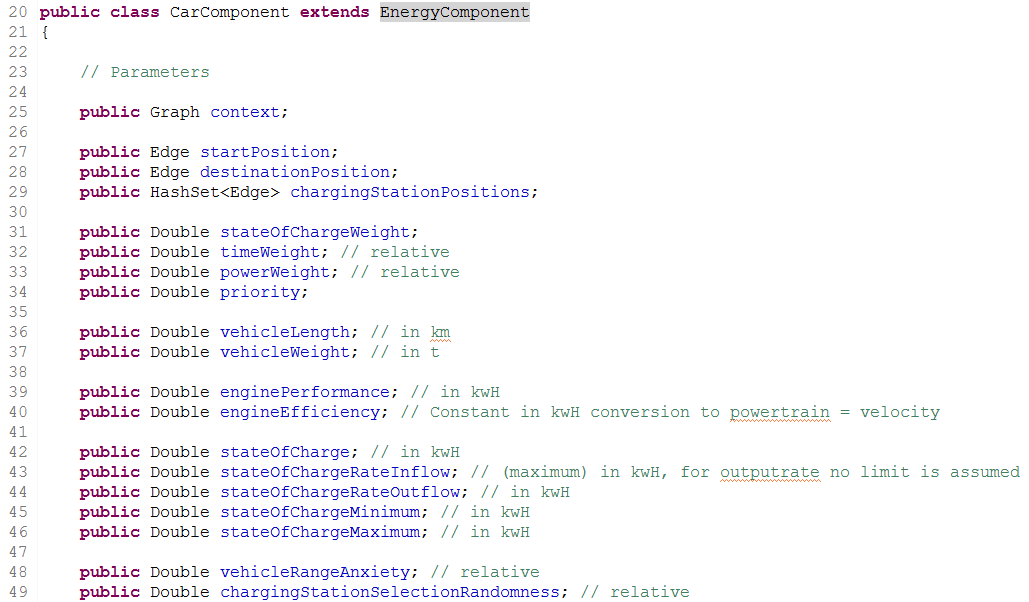
\includegraphics[width=\columnwidth]{./gfx/modeling.png}
	\caption{System modeling using regular Java classes and the Eclipse integrated development environment (IDE).}
	\label{figure:modeling}
\end{figure}

TODO

\begin{figure}[h]
	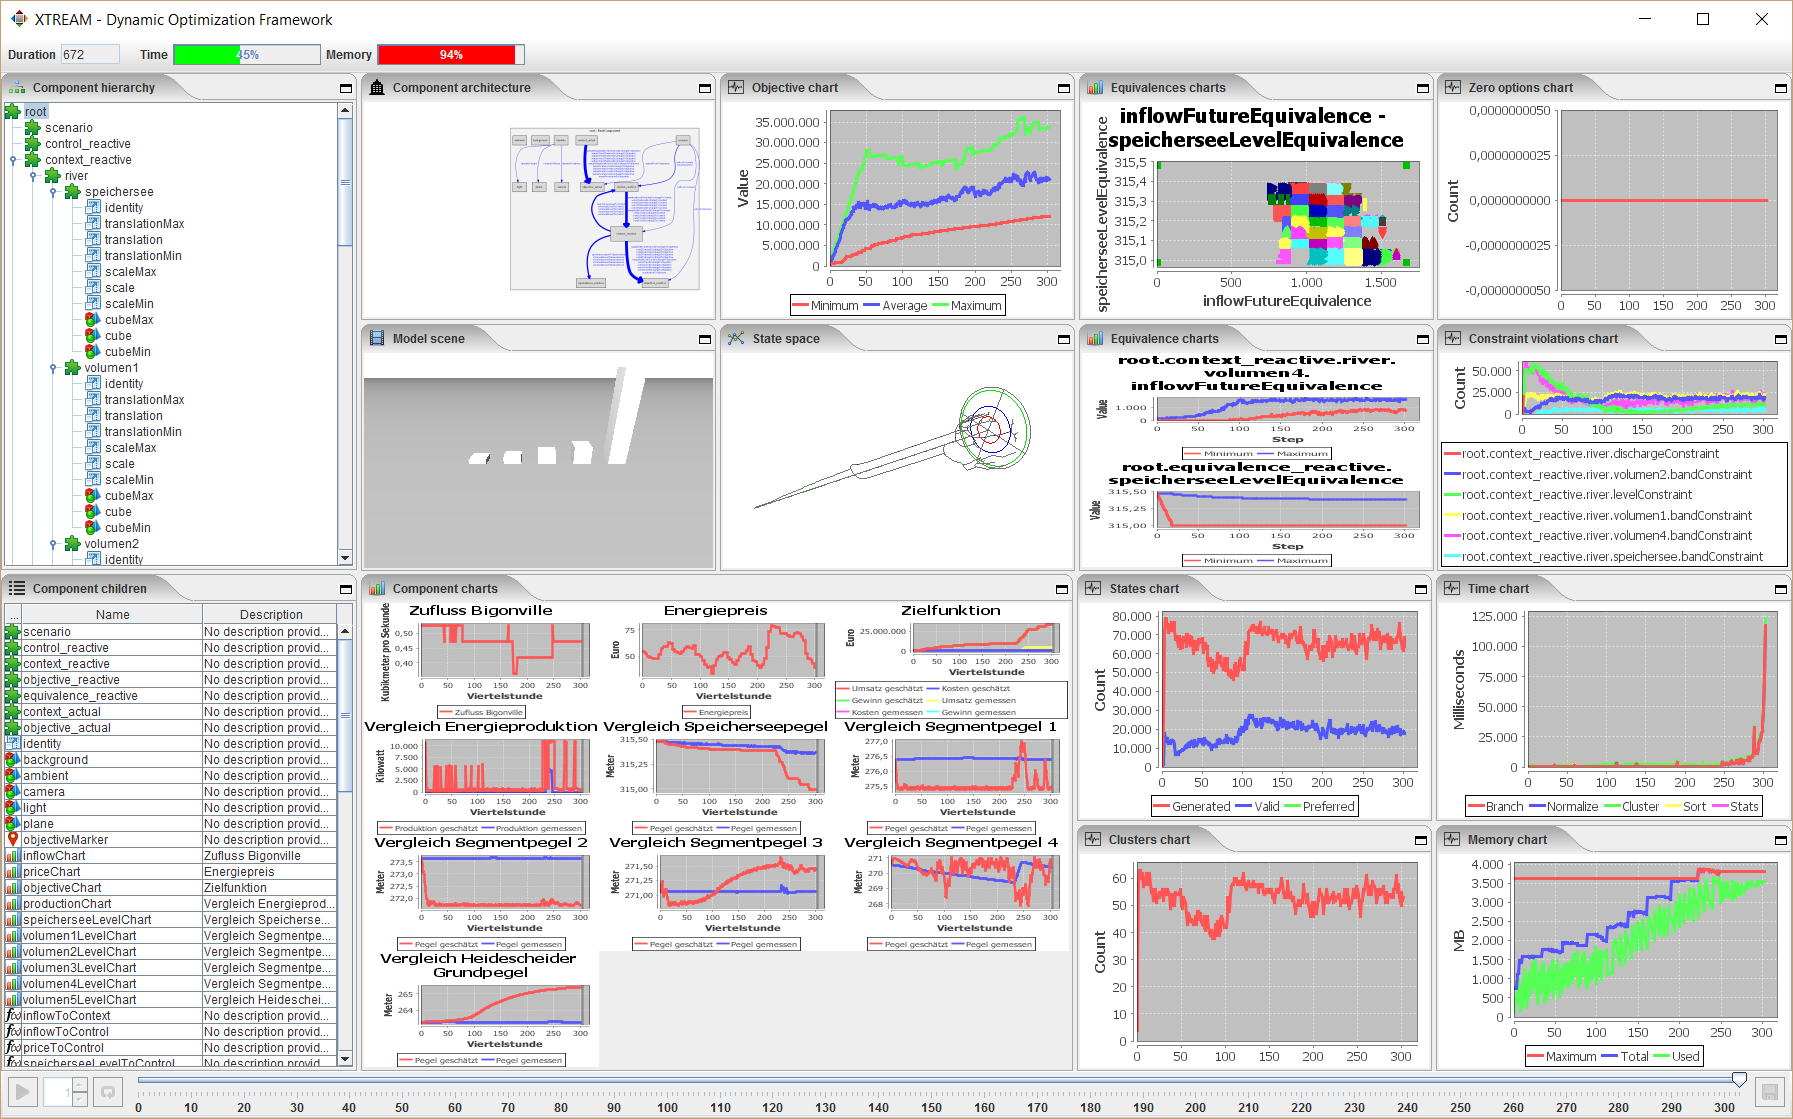
\includegraphics[width=\columnwidth]{./gfx/analysis.png}
	\caption{Model analysis using a basic approximate dynamic programming algorithm and comprehensive visualization techniques.}
	\label{figure:analysis}
\end{figure}

TODO

\subsection{Exemplary system designs}
\label{examples}

To demonstrate the proposed approach and underlying model, we propose several scenarios for commuter traffic. In each scenario, in order to reach their location of work, ten traffic participants travel between home to work locations. Travel is subject to specified time windows, which are imposed on arrival and leaving times at the specific locations, i.e. home and work. The demonstration then evaluates the behavior of typical work commute on transportation and power systems within small scale scenarios, which vary the structure of the underlying infrastructure as well as the employed objectives and constraints.

Subsequently, we evaluate our systematic approach using different traffic scenarios with different configurations varying in their respective parameters and structure of cost functions. Note that at this point we do not consider varying constraints. 


%Hence, in each time step traffic participants actions consist in selecting driving speed, time of charging, time of departure as well as route selection when driving towards their respective destination positions. 

For all scenarios in general, we employ a traffic infrastructure which is consisted of a traffic network of 20 by 5 kilometers with two possible origins and two possible destinations of travel for individual traffic participants. At its most basic level, the traffic infrastructure is consisted of a basic structure, where two origin-destination pairs are connected. We then introduce an extended traffic infrastructure, which features additional pathways, which can possibly allow for more energy-efficient or less congested routes between respective origin and destinations.

Furthermore, we employ a electric network structure, featuring a single voltage net for all consumers and producers. Then, we introduce another structure of the electric network, which distinguishes two voltage nets for each home and work consumers and producers.

\begin{figure}
	\centering
	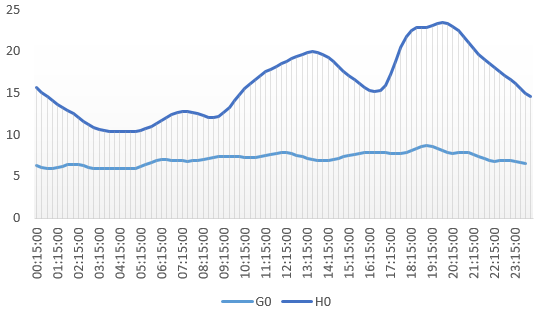
\includegraphics[width=\columnwidth]{gfx/profiles.PNG}
	\caption{Illustration of home (H0) and workplace (G0) load profiles.}
	\label{profiles}
\end{figure}

We vary scenario configuration with regard to the objective function, voltage net and traffic network structure. Subsequently we describe the according measures of variation.

\subsubsection{Objective function structure}

The objective function structure concerns the weighting and structure of individually employed objective functions. In the presented example scenarios, we vary cost functions with regard to vehicle energy-efficiency and vehicle shortest-traveling time objectives and the respective weighting of these cost functions. 

\subsubsection{Voltage net structure}
Voltage net structure is expressed by the underlying tree-like overall electric net infrastructure. More specifically, it concerns the number of employed low voltage nets for a given model excerpt. In the presented example scenarios, we alternate between assigning one or multiple distinct voltage nets to a group of consumers or producers based on their locality.

\subsubsection{Traffic network structure}
Traffic network structure concerns the number of available intersections as well as their connected segments making up the traffic infrastructure. In general, the traffic infrastructure can be changed by adding additional interactions or segments, allowing for a wider variety of resulting routes to be chosen by the traffic participants, e.g. enabling more energy-efficient or shorter routes.

\subsubsection{Results}
The results are pictured in Figure \ref{figure:examples}. 

\begin{table*}[b]
	\centering
	\renewcommand{\arraystretch}{1.3}
	\begin{tabularx}{\textwidth}{|Y|Y|Y|Y|}
		\hline
		
		\textbf{Scenario 1} & \textbf{Scenario 2} & \textbf{Scenario 3} \\
		
		\hline
		
		Energy-efficiency &
		Shortest traveling time &
		Intermediate \\
		
		\hline
		
		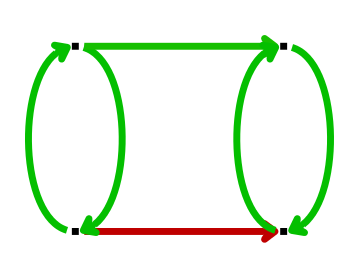
\includegraphics[width=0.20\textwidth, trim=0 0 0 -3]{gfx/Graph2.png} &
		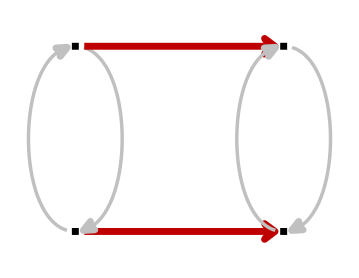
\includegraphics[width=0.20\textwidth, trim=0 0 0 -3]{gfx/Graph1.png} &
		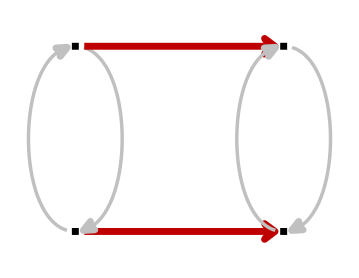
\includegraphics[width=0.20\textwidth, trim=0 0 0 -3]{gfx/Graph1.png} \\
		
		\hline
		
		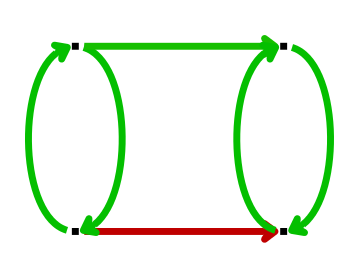
\includegraphics[width=0.20\textwidth, trim=0 0 0 -3]{gfx/Graph2.png} &
		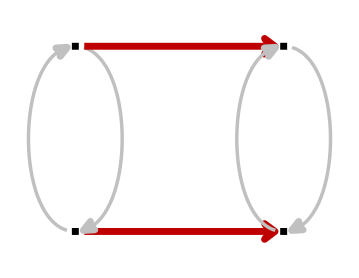
\includegraphics[width=0.20\textwidth, trim=0 0 0 -3]{gfx/Graph1.png} &
		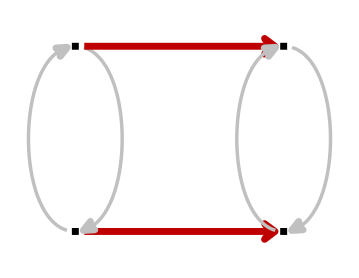
\includegraphics[width=0.20\textwidth, trim=0 0 0 -3]{gfx/Graph1.png} \\
		\hline			
	\end{tabularx}
	\caption{Traffic flow graph and power charts for different configurations.}
	\label{figure:examples}
\end{table*}